The primary objective of this stakeholder analysis is to identify all key actors, evaluate their power (influence) and interest in the project, and establish tailored management strategies to ensure seamless cooperation, secure data workflows, and mitigate political or operational resistance.

We have identified the stakeholders and divided them into four primary groups. Each group contains specific organizations, agencies, or team roles that directly interact with the system.

\subsection{Institutional Users \& Decision Makers}

This group consists of high-level government entities and civil protection agencies that rely directly on \abbr{EWAS} outputs to protect human life and manage national crises. They do not operate the satellites, but they are the primary consumers of the warning products.

\begin{itemize}
    \item \textbf{National Crisis Management \& Emergency Response Authorities:} Specific regional government security centers and sovereign security authorities within the alliance's territory, alongside their respective Ministries of the Interior. These institutions require immediate, clear data to initiate national safety protocols.
    
    \item \textbf{Emergency Warning Centers:} Operational hubs (such as civil defense headquarters and regional emergency dispatch centers) that receive the 2D tactical maps and probabilistic impact ellipses to coordinate local actions.
    
    \item \textbf{Designated Government Decision-Makers:} Ministers of Defense, Ministers of Interior, and heads of state who need high-fidelity data to make rapid geopolitical and defensive decisions during a missile crisis.
\end{itemize}

\subsection{Operational \& Technical Team}

This group includes the internal team roles responsible for the day-to-day survival, maintenance, and continuous optimization of both the Space and Ground segments. They ensure the system maintains its required 99.9\% availability.

\begin{itemize}
    \item \textbf{System Operators \& Satellite Controllers:} Tactical personnel working in a secure ground station. All tracking data from 72 \abbr{LEO} satellites across 8 orbital planes is routed via 6 \abbr{GEO} relays using Inter-Satellite Links (\abbrtext{ISL}{ISL}).
    
    \item \textbf{Subsystem \& Payload Engineers:} Responsible for satellite bus configuration, multi-orbit mechanics, fleet synchronization (6 \abbr{GEO} + 72 \abbr{LEO}), cryogenic \abbr{IR} sensor systems, and \abbr{ISL} routing protocols.
    
    \item \textbf{Data Analysts \& Software Developers:} Manage telemetry analytics pipeline, secure data warehouse, trajectory modeling, and multi-satellite data fusion algorithms.
\end{itemize}

\subsection{Industrial Suppliers \& Enablers}

These actors provide infrastructure, hardware, and logistics for deployment.

\begin{itemize}
    \item \textbf{Foreign Launch Service Providers:} Companies and regulators responsible for deploying \abbr{LEO} and \abbr{GEO} satellites into orbit.
    
    \item \textbf{Commercial Off-The-Shelf (\abbr{COTS}) Manufacturers:} Suppliers of standardized satellite components such as solar arrays, structures, and processors.
    
    \item \textbf{Specialized \abbr{ISL} \& Optical Payload Contractors:} Provide \abbr{SWIR}/\abbr{MWIR} sensors and laser/\abbr{RF} inter-satellite communication terminals.
\end{itemize}

\subsection{External Partners \& Alliances}

This group includes international stakeholders affected by the system.

\begin{itemize}
    \item \textbf{Partner Governments:} Allied nations receiving sanitized threat data via Cross-Domain Solutions (\abbr{CDS}).
    
    \item \textbf{International Alliances \& Funding Bodies:} Provide funding and require milestone tracking and stability outcomes.
    
    \item \textbf{Space Regulatory Agencies \& Traffic Management:} Manage orbital slots, \abbr{RF} allocation, and debris mitigation (\abbr{LEO} + \abbr{GEO} end-of-life operations).
    
    \item \textbf{General Public / Civilians:} Indirect beneficiaries of early warning infrastructure.
\end{itemize}

\subsection{Detailed Analysis}
The following table presents a detailed stakeholder analysis, identifying their respective levels of power and interest, key expectations and requirements, and the proposed management strategy for each stakeholder group.
\begin{longtable}{
    >{\centering\arraybackslash}p{0.025\textwidth}
    >{\raggedright\arraybackslash}p{0.14\textwidth}
    >{\centering\arraybackslash}p{0.06\textwidth}
    >{\centering\arraybackslash}p{0.08\textwidth}
    >{\raggedright\arraybackslash}p{0.30\textwidth}
    >{\raggedright\arraybackslash}p{0.32\textwidth}
}
\caption{\centering\mbox{Stakeholder Analysis and Management Strategy}}
\label{tab:stakeholder_analysis} \\
\toprule
\textbf{ID} &
\textbf{Stakeholder} &
\textbf{Power} &
\textbf{Interest} &
\textbf{Core Expectations \& Requirements} &
\textbf{Management Strategy} \\
\midrule
\endfirsthead

\multicolumn{6}{c}%
{{\tablename\ \thetable{} -- continued from previous page}} \\
\toprule
\textbf{ID} &
\textbf{Stakeholder} &
\textbf{Power} &
\textbf{Interest} &
\textbf{Core Expectations \& Requirements} &
\textbf{Management Strategy} \\
\midrule
\endhead

\midrule
\multicolumn{6}{r}{{Continued on next page}} \\
\endfoot

\bottomrule
\endlastfoot

1 &
National Crisis Management Authorities &
High &
High &
Require immediate, clear data to activate national safety protocols and coordinate civil protection across the Baltic states. &
\textbf{Manage Closely:} Conduct regular high-level operational reviews and integrate their communication protocols early. \\
\hline

2 &
Emergency Warning Centers &
High &
High &
Require end-to-end latency below 60 seconds and intuitive 2D tactical maps showing probabilistic impact ellipses. &
\textbf{Manage Closely:} Involve them deeply in the User Interface (\abbr{UI}) design phase to minimize human response latency during crisis conditions. \\
\hline

3 &
Designated Government Decision-Makers &
High &
High &
Expect highly reliable decision-support information and strict assurance that \abbr{EWAS} remains a non-offensive, defensive civil asset. &
\textbf{Manage Closely:} Provide high-level technical updates emphasizing compliance with civil protection boundaries. \\
\hline

4 &
System Operators \& Satellite Controllers &
High &
High &
Require 99.9\% system availability, high-fidelity visualization tools, and a streamlined single-station ground interface receiving a continuous data stream routed from the 72 \abbr{LEO} satellites via the 6 \abbr{GEO} relays. &
\textbf{Manage Closely:} Include them in \abbr{HIL} simulations that test data handovers and routing between the shifting \abbr{LEO} and fixed \abbr{GEO} layers. \\
\hline

5 &
Subsystem \& Payload Engineers &
Low &
High &
Require stable requirements to manage multi-orbit fleet synchronization (6 \abbr{GEO} + 72 \abbr{LEO} across 8 orbital planes), complex tracking geometry from 1,200 km, and structural radiation shielding. &
\textbf{Keep Informed:} Establish clear communication channels between technical layers to ensure seamless hardware and dual-orbit integration. \\
\hline

6 &
Data Analysts \& Software Developers &
Low &
High &
Require access to the secure data warehouse to refine algorithms capable of fusing overlapping trajectory data from multiple \abbr{LEO} satellites simultaneously. &
\textbf{Keep Informed:} Provide structured access to post-event data logs to support continuous software refinement and false-alarm reduction. \\
\hline

7 &
Foreign Launch Service Providers &
High &
Low &
Demand strict compliance with launch vehicle safety regulations, payload dimensions, and export control laws. &
\textbf{Keep Satisfied:} Handle as a major supply chain risk. Secure complex, multi-launch contracts needed to deploy 72 \abbr{LEO} satellites across 8 orbital planes, likely through multiple rideshare launches, and 6 heavy \abbr{GEO} satellites. \\
\hline

8 &
\abbr{COTS} Manufacturers &
Low &
High &
Require clear technical interface specifications and timely milestone payments for standardized, mass-produced components to support the 72 satellite \abbr{LEO} fleet. &
\textbf{Keep Informed:} Maintain strict quality assurance monitoring during the high-volume component procurement and integration phases. \\
\hline

9 &
Specialized \abbr{ISL} \& Optical Payload Contractors &
Low &
High &
Require precise technical profiles to manufacture 72 sets of high-speed tracking telescopes (\abbr{SWIR}/\abbr{MWIR}) and reliable, dynamic laser/\abbr{RF} Inter-Satellite Link terminals. &
\textbf{Keep Informed:} Maintain intense engineering coordination to ensure rapid data cross-linking between fast-moving \abbrtext{LEO}{LEOs} and stationary \abbr{GEO} networks. \\
\hline

10 &
Baltic Partner Governments &
Low &
High &
Expect controlled access to threat telemetry and launch archives to enhance their own national resilience and regional security planning. &
\textbf{Keep Informed:} Utilize secure Cross-Domain Solutions (\abbr{CDS}) to safely share sanitized data without exposing core system vulnerabilities. \\
\hline

11 &
International Alliances \& Funding Bodies (\abbr{NATO} / \abbr{EU}) &
Low &
High &
Expect efficient use of dual-use resources, strict project milestone tracking, and clear alignment with regional civil protection frameworks. &
\textbf{Keep Informed:} Provide periodic progress reports and financial audits to secure long-term institutional backing. \\
\hline

12 &
Space Regulatory Agencies \& Traffic Management &
High &
Low &
Demand compliance with radio frequency allocations for dense \abbr{ISL} networks, safe positioning within crowded \abbr{GEO} slots, and active space debris mitigation at 1200 km (\abbr{LEO} end-of-life disposal). &
\textbf{Keep Satisfied:} Submit complex orbital slot applications and regulatory frequency coordination paperwork very early in the system design phase. \\
\hline

13 &
General Public / Civilians &
Low &
Low &
Expect general national safety and infrastructure resilience without direct operational awareness of the satellite layers. &
\textbf{Monitor:} Track broader public trust metrics in national defense warning infrastructures; no direct communication or marketing needed. \\
\hline
\end{longtable}


\subsection{Stakeholder Matrix}
Figure~\ref{fig:ewas_matrix} illustrates the distribution of stakeholders across the power--interest matrix according to their respective levels of power and interest.
\begin{figure}[H]
    \centering
    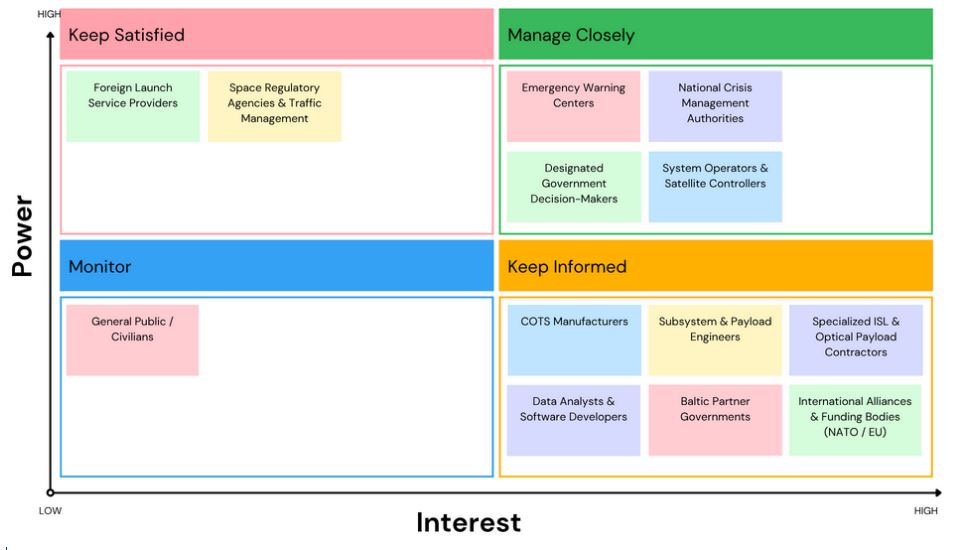
\includegraphics[width=0.85\textwidth]{Figures/ewas_matrix.png}
    \caption{Stakeholder power--interest matrix.}
    \label{fig:ewas_matrix}
\end{figure}


\subsection{Stakeholder Management Synthesis}

The stakeholder analysis highlights four main operational focus areas:

\begin{itemize}
    \item \textbf{Manage Closely (High Power, High Interest):} Institutional users and operators requiring low-latency decision support and intuitive interfaces during crisis conditions.
    
    \item \textbf{Keep Informed (Low Power, High Interest):} Engineers, developers, and suppliers ensuring continuous system development and integration across \abbr{LEO} and \abbr{GEO} layers.
    
    \item \textbf{Keep Satisfied (High Power, Low Interest):} Launch providers and regulatory agencies requiring compliance and early coordination.
    
    \item \textbf{Monitor (Low Power, Low Interest):} General public, with focus on long-term trust in national warning infrastructure.
\end{itemize}